\documentclass{standalone}

\usepackage{tikz}

\usetikzlibrary{calc}

\begin{document}
  %noformat{
  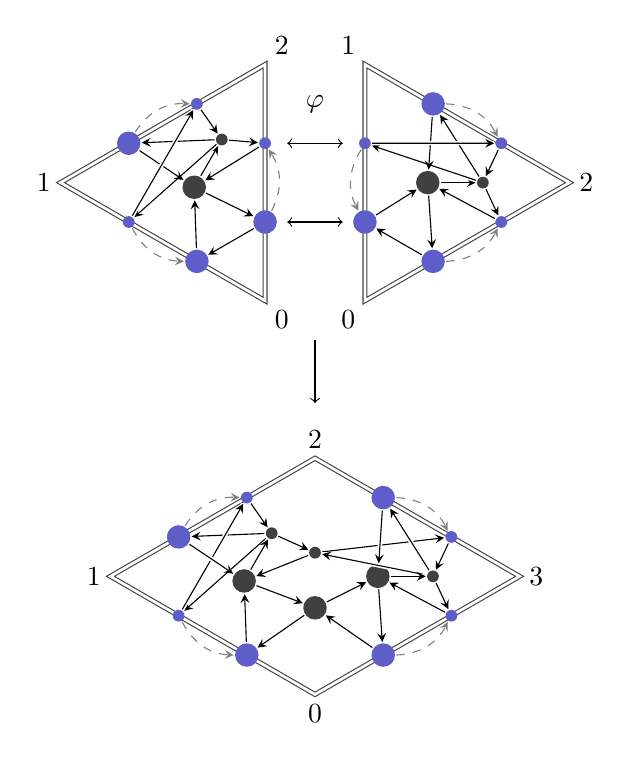
\begin{tikzpicture}
    \tikzstyle{v1} = [circle, outer sep=0.5pt, fill, inner sep=1.5pt]
    \tikzstyle{v2} = [circle, outer sep=0.5pt, fill, inner sep=3.0pt]
    \tikzstyle{unf} = [color=darkgray]
    \tikzstyle{frz} = [color=blue!60!darkgray!70]
    \tikzstyle{r} = [color=red!70!darkgray!70]
    \tikzstyle{e} = [->, >={stealth}, preaction={draw=white, -, ultra thick}]
    \tikzstyle{b} = [fill, fill opacity=0.0, circle, outer sep=0.5pt, inner sep=1.5pt]
    \tikzstyle{te} = [color=darkgray, double distance=1pt]
    \tikzstyle{h} = [dashed, color=gray, ->, >={stealth}]

    % Left hand side, left quiver
    \begin{scope}[shift={(0,0)}]
      \coordinate[label={300:$0$}] (l_0) at (-60:1.7321);
      \coordinate[label={180:$1$}] (l_1) at (180:1.7321);
      \coordinate[label={ 60:$2$}] (l_2) at ( 60:1.7321);

      \draw[te] (l_0) -- (l_1) -- (l_2) -- cycle;
 
      \node[v2, frz] (A1) at ($ (l_0) + (150:1.0) $) {};
      \node[v1, frz] (A2) at ($ (l_0) + (150:2.0) $) {};

      \node[v2, frz] (C1) at ($ (l_0) + ( 90:1.0) $) {};
      \node[v1, frz] (C2) at ($ (l_0) + ( 90:2.0) $) {};

      \node[v2, frz] (B1) at ($ (l_1) + ( 30:1.0) $) {};
      \node[v1, frz] (B2) at ($ (l_1) + ( 30:2.0) $) {};

      \node[v2, unf] (v1) at ($ (l_2) + (240:1.8)$) {};
      \node[v1, unf] (v2) at ($ (l_2) + (240:1.1)$) {};

      \draw[h] (A2) to[bend right] (A1);
      \draw[h] (B1) to[bend left] (B2);
      \draw[h] (C1) to[bend right] (C2);

      \draw[e] (v1) -- (v2);
      \draw[e] (v1) -- (C1);
      \draw[e] (v2) -- (B1);
      \draw[e] (v2) -- (C2);
      \draw[e] (v2) -- (A2);
      \draw[e] (B1) -- (v1);
      \draw[e] (B2) -- (v2);
      \draw[e] (C1) -- (A1);
      \draw[e] (C2) -- (v1);
      \draw[e] (A1) -- (v1);
      \draw[e] (A2) -- (B2);
    \end{scope}

    % Left hand side, right quiver
    \begin{scope}[shift={(3,0)}]
      \coordinate[label={240:$0$}] (r_0) at (240:1.7321);
      \coordinate[label={120:$1$}] (r_1) at (120:1.7321);
      \coordinate[label={  0:$2$}] (r_2) at (  0:1.7321);

      \draw[te] (r_0) -- (r_1) -- (r_2) -- cycle;
 
      \node[v2, frz] (A1) at ($ (r_0) + ( 90:1.0) $) {};
      \node[v1, frz] (A2) at ($ (r_0) + ( 90:2.0) $) {};

      \node[v2, frz] (C1) at ($ (r_0) + ( 30:1.0) $) {};
      \node[v1, frz] (C2) at ($ (r_0) + ( 30:2.0) $) {};

      \node[v2, frz] (B1) at ($ (r_1) + (-30:1.0) $) {};
      \node[v1, frz] (B2) at ($ (r_1) + (-30:2.0) $) {};

      \node[v2, unf] (v1) at ($ (r_2) + (180:1.8)$) {};
      \node[v1, unf] (v2) at ($ (r_2) + (180:1.1)$) {};

      \draw[h] (A2) to[bend right] (A1);
      \draw[h] (B1) to[bend left] (B2);
      \draw[h] (C1) to[bend right] (C2);

      \draw[e] (v1) -- (v2);
      \draw[e] (v1) -- (C1);
      \draw[e] (v2) -- (B1);
      \draw[e] (v2) -- (C2);
      \draw[e] (v2) -- (A2);
      \draw[e] (B1) -- (v1);
      \draw[e] (B2) -- (v2);
      \draw[e] (C1) -- (A1);
      \draw[e] (C2) -- (v1);
      \draw[e] (A1) -- (v1);
      \draw[e] (A2) -- (B2);
    \end{scope}

    % Oh, what a tangled web we weave...
    \coordinate (xa) at ($ (0,0) + (-60:1.7321) + ( 90:1.0) $);
    \coordinate (xb) at ($ (3,0) + (240:1.7321) + ( 90:1.0) $);
    \coordinate (ya) at ($ (0,0) + (-60:1.7321) + ( 90:2.0) $);
    \coordinate (yb) at ($ (3,0) + (240:1.7321) + ( 90:2.0) $);
    \draw[<->] ($ (xa) + (0:8pt) $) -- ($ (xb) + (180:8pt) $);
    \draw[<->] ($ (ya) + (0:8pt) $) -- ($ (yb) + (180:8pt) $);
    \node at ($ (ya)!0.5!(yb) + (90:0.5) $) {$\varphi$};

    \begin{scope}[shift={(1.5,-5)}]
      \coordinate[label=270:{$0$}] (q_0) at (270:1.5);
      \coordinate[label=180:{$1$}] (q_1) at (180:2.598);
      \coordinate[label= 90:{$2$}] (q_2) at ( 90:1.5);
      \coordinate[label=  0:{$3$}] (q_3) at (  0:2.598);

      \draw[te] (q_0) -- (q_1) -- (q_2) -- (q_3) -- cycle;
 
      \node[v2, frz] (D1) at    ($ (q_0) + (150:1.0) $) {};
      \node[v1, frz] (D2) at    ($ (q_0) + (150:2.0) $) {};

      \node[v2, frz] (E1) at    ($ (q_1) + ( 30:1.0) $) {};
      \node[v1, frz] (E2) at    ($ (q_1) + ( 30:2.0) $) {};

      \node[v2, frz] (F1) at    ($ (q_2) + (-30:1.0) $) {};
      \node[v1, frz] (F2) at    ($ (q_2) + (-30:2.0) $) {};

      \node[v2, frz] (G1) at    ($ (q_0) + ( 30:1.0) $) {};
      \node[v1, frz] (G2) at    ($ (q_0) + ( 30:2.0) $) {};

      \node[v2, unf] (w11) at ($ (q_3) + (180:1.8)$) {};
      \node[v1, unf] (w21) at ($ (q_3) + (180:1.1)$) {};
      \node[v2, unf] (w12) at ($ (q_0) + ( 90:1.1)$) {};
      \node[v1, unf] (w22) at ($ (q_0) + ( 90:1.8)$) {};
      \node[v2, unf] (w13) at ($ (q_2) + (240:1.8)$) {};
      \node[v1, unf] (w23) at ($ (q_2) + (240:1.1)$) {};

      \draw[h]  (D2) to[bend right] (D1);
      \draw[h]  (E1) to[bend left]  (E2);
      \draw[h]  (F1) to[bend left]  (F2);
      \draw[h]  (G1) to[bend right] (G2);

      \draw[e] (D1) -- (w13);
      \draw[e] (w23) -- (w22);
      \draw[e] (w23) -- (D2);
      \draw[e] (w23) -- (E1);
      \draw[e] (w12) -- (D1);
      \draw[e] (w12) -- (w11);
      \draw[e] (w22) -- (w13);
      \draw[e] (w22) -- (F2);
      \draw[e] (E2) -- (w23);
      \draw[e] (D2) -- (E2);
      \draw[e] (w13) -- (w23);
      \draw[e] (w13) -- (w12);
      \draw[e] (E1) -- (w13);
      \draw[e] (w21) -- (w22);
      \draw[e] (w21) -- (G2);
      \draw[e] (w21) -- (F1);
      \draw[e] (G1) -- (w12);
      \draw[e] (G2) -- (w11);
      \draw[e] (F2) -- (w21);
      \draw[e] (w11) -- (w21);
      \draw[e] (w11) -- (G1);
      \draw[e] (F1) -- (w11);
    \end{scope}

    \draw[->] ($ (q_2) + ( 90:1.5) $) -- ($ (q_2) + ( 90:0.7) $);


  \end{tikzpicture}
  %}noformat
\end{document}
